\renewcommand*{\arraystretch}{1.1}

\subsection*{BI / read / 16}
\label{section:bi-read-16}

% change \emph{} to use sans-serif font
\let\oldemph\emph
\renewcommand{\emph}[1]{\footnotesize \sf #1}

\renewcommand{\currentQueryCard}{16}
\marginpar{
	\raggedleft
	\vspace{0.22ex}

    \queryRefCard{bi-read-01}{BI}{1}\\
    \queryRefCard{bi-read-02}{BI}{2}\\
    \queryRefCard{bi-read-03}{BI}{3}\\
    \queryRefCard{bi-read-04}{BI}{4}\\
    \queryRefCard{bi-read-05}{BI}{5}\\
    \queryRefCard{bi-read-06}{BI}{6}\\
    \queryRefCard{bi-read-07}{BI}{7}\\
    \queryRefCard{bi-read-08}{BI}{8}\\
    \queryRefCard{bi-read-09}{BI}{9}\\
    \queryRefCard{bi-read-10}{BI}{10}\\
    \queryRefCard{bi-read-11}{BI}{11}\\
    \queryRefCard{bi-read-12}{BI}{12}\\
    \queryRefCard{bi-read-13}{BI}{13}\\
    \queryRefCard{bi-read-14}{BI}{14}\\
    \queryRefCard{bi-read-15}{BI}{15}\\
    \queryRefCard{bi-read-16}{BI}{16}\\
    \queryRefCard{bi-read-17}{BI}{17}\\
    \queryRefCard{bi-read-18}{BI}{18}\\
    \queryRefCard{bi-read-19}{BI}{19}\\
    \queryRefCard{bi-read-20}{BI}{20}\\
    \queryRefCard{bi-read-21}{BI}{21}\\
    \queryRefCard{bi-read-22}{BI}{22}\\
    \queryRefCard{bi-read-23}{BI}{23}\\
    \queryRefCard{bi-read-24}{BI}{24}\\
    \queryRefCard{bi-read-25}{BI}{25}\\
}



\noindent\begin{tabularx}{\queryCardWidth}{|>{\queryPropertyCell}p{\queryPropertyCellWidth}|X|}
	\hline
	query & BI / read / 16 \\ \hline
%
	title & Experts in social circle
 \\ \hline
%
	pattern & \hfill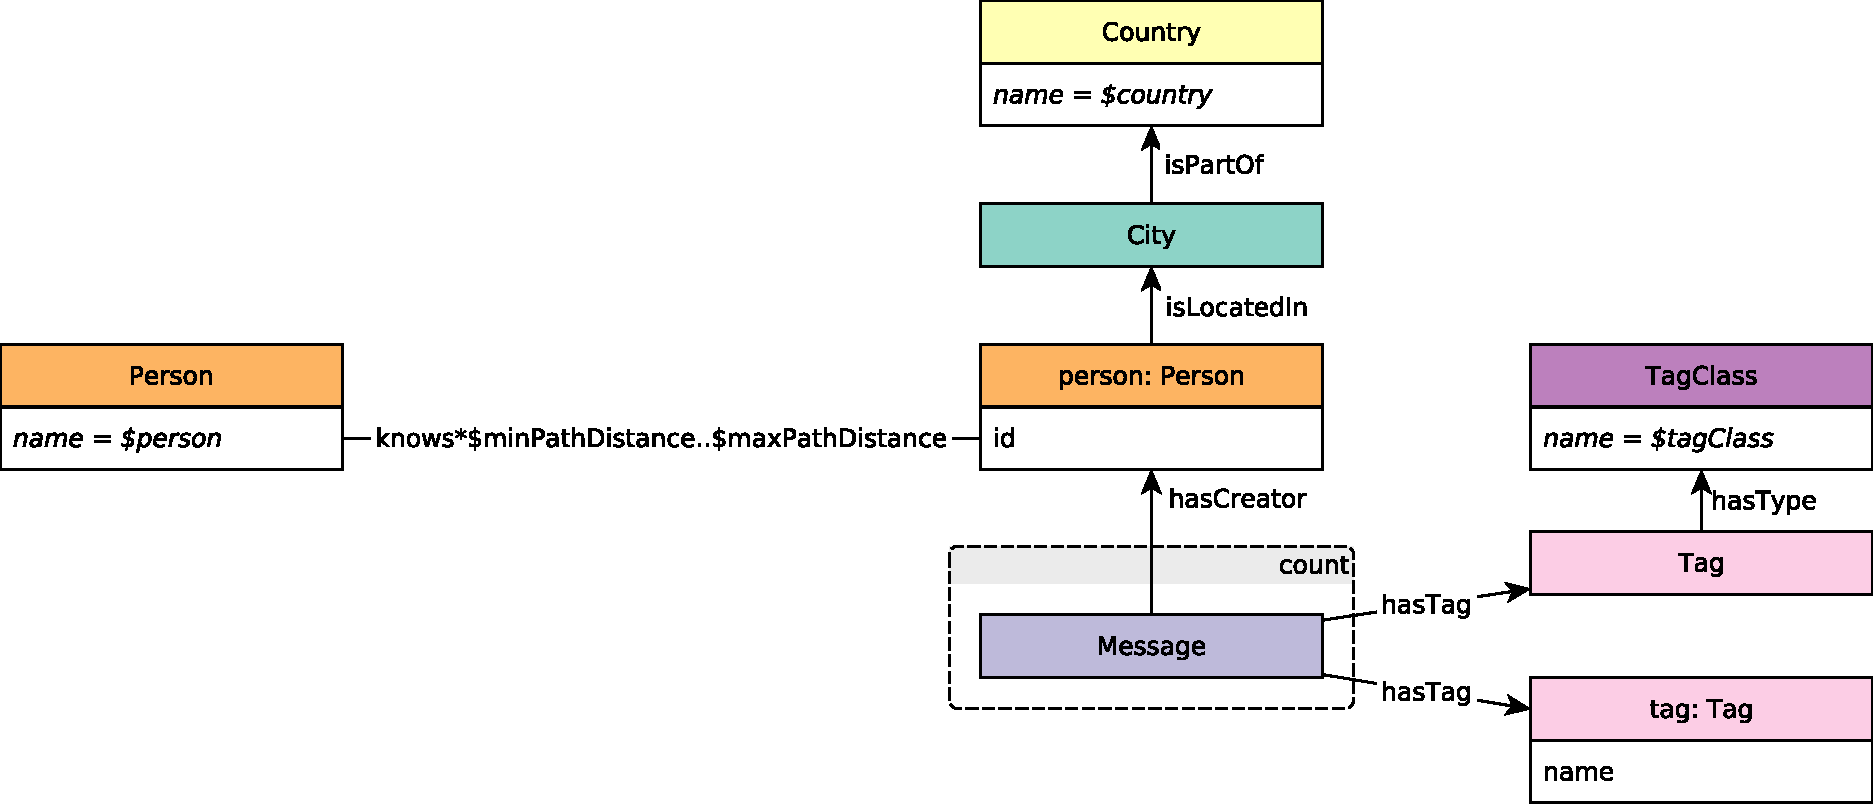
\includegraphics[scale=\patternscale,margin=0cm .2cm]{patterns/bi-read-16}\hfill\vadjust{} \\ \hline
%
	desc. & Given a \emph{Person}, find all other \emph{Persons} that live in a
given \texttt{country} and are connected to given \emph{Person} by a
transitive path with length in range
\texttt{{[}minPathDistance,\ maxPathDistance{]}} through the
\emph{knows} relation.

In the path, an edge can be only traversed once while nodes can be
traversed multiple times.

For each of these \emph{Persons}, retrieve all of their \emph{Messages}
that contain at least one \emph{Tag} belonging to a given
\emph{TagClass} (direct relation not transitive). For each
\emph{Message}, retrieve all of its \emph{Tags}.

Group the results by \emph{Persons} and \emph{Tags}, then count the
\emph{Messages} by a certain \emph{Person} having a certain \emph{Tag}.
 \\ \hline
%
	
		params &
		\innerCardVSpace{\begin{tabularx}{\attributeCardWidth}{|>{\paramNumberCell}c|>{\varNameCell}M|>{\typeCell}m{\typeWidth}|Y|} \hline
		$\mathsf{1}$ & personId
 & 64-bit Integer
 &  \\ \hline
		$\mathsf{2}$ & country
 & String
 &  \\ \hline
		$\mathsf{3}$ & tagClass
 & String
 &  \\ \hline
		$\mathsf{4}$ & minPathDistance
 & 32-bit Integer
 &  \\ \hline
		$\mathsf{5}$ & maxPathDistance
 & 32-bit Integer
 &  \\ \hline
		\end{tabularx}}\innerCardVSpace \\ \hline
	
%
	
		result &
		\innerCardVSpace{\begin{tabularx}{\attributeCardWidth}{|>{\resultNumberCell}c|>{\varNameCell}M|>{\typeCell}m{\typeWidth}|>{\resultOriginCell}c|Y|} \hline
		$\mathsf{1}$ & person.id & 64-bit Integer & R &
				 \\ \hline
		$\mathsf{2}$ & tag.name & String & R &
				 \\ \hline
		$\mathsf{3}$ & messageCount & 32-bit Integer & A &
				Number of \emph{Messages} created by that \emph{Person} containing that
\emph{Tag}
 \\ \hline
		\end{tabularx}}\innerCardVSpace \\ \hline
	
%
	
		sort		&
		\innerCardVSpace{\begin{tabularx}{\attributeCardWidth}{|>{\sortNumberCell}c|>{\varNameCell}M|>{\directionCell}c|Y|} \hline
		$\mathsf{1}$ & messageCount
 & $\desc
$ &  \\ \hline
		$\mathsf{2}$ & tag.name
 & $\asc
$ &  \\ \hline
		$\mathsf{3}$ & person.id
 & $\asc
$ &  \\ \hline
		\end{tabularx}}\innerCardVSpace \\ \hline
	%
	limit & 100 \\ \hline
	%
	CPs &
	\multicolumn{1}{>{\raggedright}l|}{
		\chokePoint{1.2}, 
		\chokePoint{1.4}, 
		\chokePoint{2.3}, 
		\chokePoint{2.4}, 
		\chokePoint{3.3}, 
		\chokePoint{7.1}, 
		\chokePoint{7.2}, 
		\chokePoint{7.3}
		} \\ \hline
	%
	%
\end{tabularx}
\queryCardVSpace

% change \emph back to the old one
\renewcommand{\emph}[1]{\oldemph{#1}}